%!TEX root = ../Lab_report.tex
%*******************************************************************************
%*********************************** Analysis Chapter *****************************
%*******************************************************************************
\section{Free-Solution DNA electrophoresis}
Electrophoresis is an experimental technique used to separate charged molecules like polyelectrolyte chains by making use of the interaction between the particles and external electric fields. In a solution with counterions, the dynamics of a charged polymer chain is governed by electrostatic interactions between polymers and counterions as well as hydrodynamic interactions. We investigate the dynamical properties of polyelectrolytes of different lengths in a bulk solution using coarse grained Molecular Dynamics simulations with electrostatics and hydrodynamical interactions. All simulations were carried out with ESPResSo \cite{weik2019espresso}. Electrostatic interactions are modelled efficiently with the P3M method with periodic boundary conditions. The Lattice-Boltzmann method (LBM) is employed to model hydrodynamical interactions.

\subsection{System setup}
We conducted several simulations of a system with equal parameters except the number of monomers $N$ on the polyelectrolyte chain. In every simulation the system consisted of $N$ (where $1\le N \ge 32$)monomers connected by bonded interactions modelled with a FENE potential. Furthermore, $N$ counterions are placed at random positions in the simulation box. All simulated particles exhibited short ranged repulsive interactions, modelled by a WCA potential and long ranged electrostatic interactions, where a Bjerrum length of $l_\text{B} = 2.84$ in reduced units was chosen. The box size of the cubic simulation box was chosen such that the mean concentration of monomers in the solution was kept constant at $\SI{5}{\milli M}$. To remove overlap between all particles in the system, first, a total of $2000$ gradient based energy minimization steps were performed to remove overlap between all particles in the system. Subsequently, after activating electrostatic and hydrodynamic interactions, the system was equilibrated for $\SI{5e5}{}$ integration steps. During the production run, we sampled data every integration step for a total of $\SI{5e6}{}$ steps. Figure \ref{fig:vmd} displays a snapshot during the simulation of a polymer chain with $N=32$ after equilibration.
\begin{figure}[H]
	\centering
	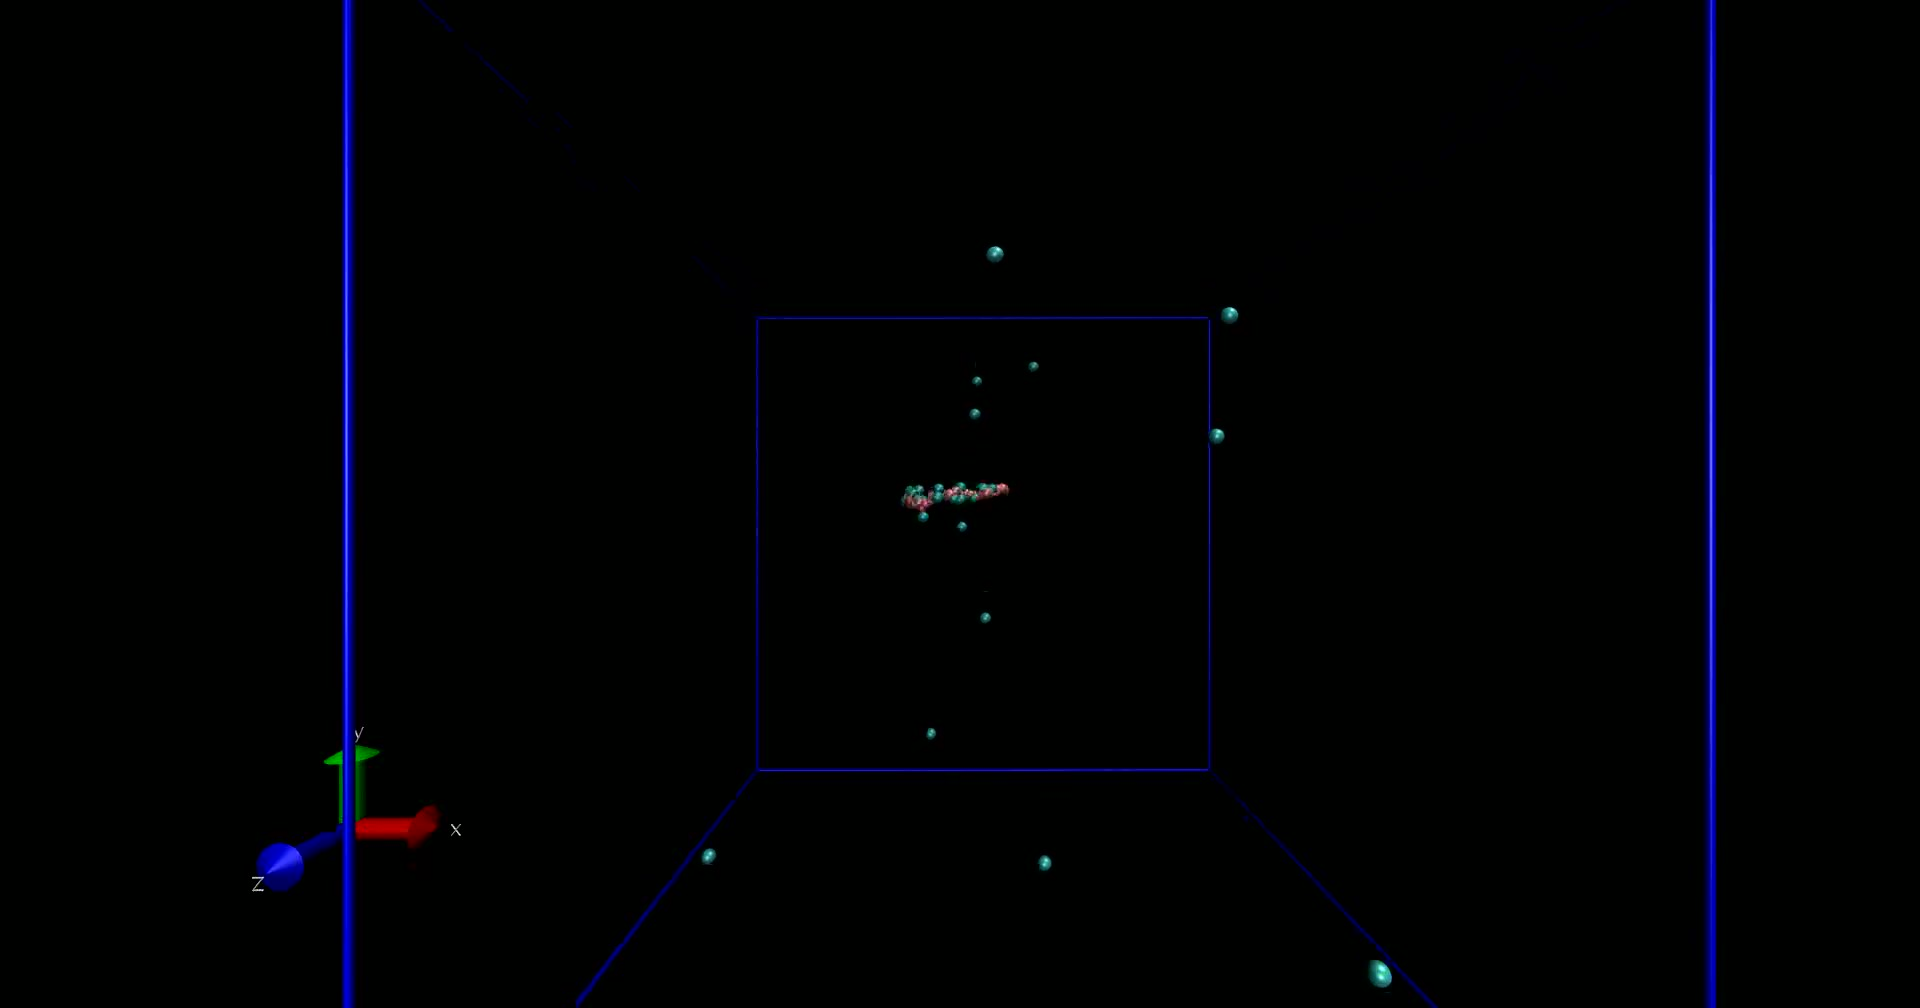
\includegraphics[width=\columnwidth]{Analysis_1/VMD_visualization}
	\captionsetup{width=\columnwidth}
	\caption{Visualization of a simulated polyelectrolyte with a chain length of 32.}
	\label{fig:vmd}
\end{figure}
\subsection{Results}
The diffusion coefficient $D$ is a critical dynamic observable of our system. Theoretically, in the Zimm model, one expects the $D$ to show a length-scaling behavior with $D \propto N^{-\nu}$ (where $\nu < 1$) in the presence of hydrodynamic interactions. It can be computed by integrating over the velocity auto-correlation  function of the polymer center of masses as
\begin{equation}
	D = \frac{1}{3} \int_{0}^{\infty} \langle \vec{v}_\text{cm}(t) \cdot \vec{v}_\text{cm}(0) \rangle dt.
\end{equation}
Since we only have access to a limited time frame of sampled velocities, the integration has to have an upper limit. Fortunately, the velocity auto-correlation function behaves as an exponentially decaying function for large times. This ensures that the error from cutting off the integral earlier is very small. In Figure ??? the computed diffusion coefficients are plotted over the number of monomers from different simulations.

Moreover, we can compute the effective charge of the polyelectrolyte chain in the presence of condensed counterions. Since, in our system, the Manning parameter is $\xi = l_b / b$, we expect a fraction of the total number of counterions to be always condensed onto the polyelectrolyte due to electrostatic interactions. Manning theory predicts the number of condensed counterions to be $f_text{CI} = 1 - 1/\xi$, hence; the effective charge on the polymer is expected to be $N_\text{CI} = (1-1/\xi)N$.